% Valentino Vranic
% Metody inzinierskej prace 2012/13

\documentclass{beamer}

% \usetheme{Warsaw}
% \usetheme{Antibes}
\usetheme{JuanLesPins}
% \usetheme{Goettingen} 

% \usecolortheme{seahorse}
% \usecolortheme{dolphin}
\usecolortheme{rose}
% \usecolortheme{dove}
% http://deic.uab.es/~iblanes/beamer_gallery/index_by_color.html
%\usecolortheme{beaver}

%\useoutertheme[]{sidebar}
 
\setbeamercovered{transparent}

\usepackage[english]{babel}
\usepackage[T1]{fontenc}
\usepackage[utf8]{inputenc}
\usepackage{url}

\usepackage{listings}
\usepackage{tikz}

\usetikzlibrary{automata, positioning, arrows}
\usetikzlibrary{arrows.meta}
\usepackage{pgfplots} 
\pgfplotsset{compat=1.18}
\usepgfplotslibrary{external}
% \tikzexternalize

% \lstset{language=C++,basicstyle=\fontsize{8}{9.6}\selectfont,showstringspaces=false,columns=fullflexible,identifierstyle=\ttfamily,keywordstyle=\bfseries,showstringspaces=false,columns=fullflexible}
%\lstset{language=C,basicstyle=\fontsize{10.5}{12.6}\selectfont,identifierstyle=\ttfamily,keywordstyle=\bfseries,showstringspaces=false,columns=fixed}

\def\BibTeX{\textsc{Bib}\kern-.08em\TeX} 

\newcommand{\footcite}[1]{\footnote{\tiny #1}}
\newcommand{\umlet}{.5}
\newcommand{\emp}[1]{\textit{\alert{#1}}}
\newcommand{\kw}[1]{\mbox{\textbf{#1}}}
\newcommand{\id}[1]{\texttt{#1}}
\newcommand{\stl}{\guillemotleft}
\newcommand{\str}{\guillemotright}

\newcommand{\lsti}{\lstinline[basicstyle=\fontsize{10.5}{12.1}\selectfont]}

\newcommand{\ssection}[1]{
	\section{#1}
	\begin{frame}[fragile=singleslide]\frametitle{}
	\Huge #1
	\end{frame}
}

\newcommand{\ssectionn}[1]{
	\section*{#1}
	\begin{frame}[fragile=singleslide]\frametitle{}
	\Huge #1
	\end{frame}
}

\newenvironment{program}{\begin{beamercolorbox}[rounded=true,shadow=true]{block body}\vspace{-4mm}}{\vspace{-2mm}\end{beamercolorbox}}

\setbeamercolor{fvystup}{fg=white,bg=black}
\newenvironment{vystup}{\begin{beamercolorbox}[rounded=true,shadow=true]{fvystup}}{\end{beamercolorbox}}

\newenvironment{poznamka}{\begin{beamercolorbox}[rounded=true,shadow=false]{block body}}{\end{beamercolorbox}}

\setbeamertemplate{footline}[page number]
{
%\insertpagenumber
% \begin{beamercolorbox}{section in head/foot}
%\vskip2pt\insertnavigation{\paperwidth}\vskip2pt
%\end{beamercolorbox}%
}



\author{Roman Gajdoš}
%\url{www.fiit.stuba.sk/~vranic}, \url{vranic@fiit.stuba.sk}}
%{\tiny \url{www.fiit.stuba.sk/~vranic}, \url{vranic@fiit.stuba.sk}}
\institute{
	Ústav informatiky, informačných systémov a softvérového inžinierstva\\
	Fakulta informatiky a informačných technológií\\
	Slovenská technická univerzita v Bratislave}

\subtitle{\vspace{3mm} Engineering Methods 2023/2024}

\title{Overview and Analysis of GPU Acceleration for Regular Expressions
}

\date{\footnotesize 27. november 2023}




\begin{document}

\begin{frame}[fragile=singleslide]
	\titlepage
\end{frame}


\begin{frame}[fragile=singleslide]\frametitle{O čom to je}
	Ešte pre prehľadom prezentácie sa zvyčajne uvádza motivácia.

	Bežne sa aj tu používajú odrážky, ale tento text je naschvál uvedený bez odrážok. Niekedy môže byť potrebné uviesť aj citáty\ldots{}

	Toto je len príklad slajdov. Ako urobiť dobrú prezentáciu bolo vysvetlené na prednáške.
\end{frame}


\begin{frame}[fragile=singleslide]\frametitle{Outline}
	\tableofcontents
\end{frame}


\section{Background}
% príkaz \ssection by vytvoril zvláštný slajd s názvom časti - v krátkych prezentáciách to prekáža, lebo oberá o čas

\begin{frame}[fragile=singleslide]\frametitle{Background}
	\begin{columns}
		\begin{column}{0.45\textwidth}
			\begin{itemize}
				\item Regular expressions
				      \begin{itemize}
					      \item Finite state automata
					      \item DFA and NFA
				      \end{itemize}
				\item GPU
				      \begin{itemize}
					      \item Large memory bandwidth and parallelism
					      \item CUDA and OpenCL
				      \end{itemize}
			\end{itemize}
		\end{column}

		\begin{column}{0.55\textwidth}
			\begin{figure}[h!]
				\tikzset{
					->, % makes the edges directed
					>=stealth', % makes the arrow heads bold
					node distance=3cm, % specifies the minimum distance between two nodes. Change if necessary.
					every state/.style={thick, fill=gray!10}, % sets the properties for each ’state’ node
					initial text=$ $, % sets the text that appears on the start arrow
				}
				\scalebox{.45}{
					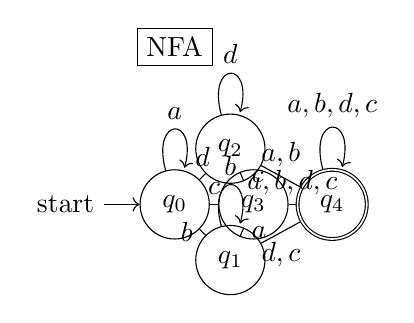
\begin{tikzpicture}
						\node[draw] at (0,2) {NFA};
						\node[state, initial] (q0) {$q_0$};
						\node[state, below right of=q0] (q1) {$q_1$};
						\node[state, above right of=q0] (q2) {$q_2$};
						\node[state, right of=q0] (q3) {$q_3$};
						\node[state, accepting, right of=q3] (q4) {$q_4$};
						\draw (q0) edge[loop above] node{$a$} (q0)
						(q0) edge[right,above] node{$c$} (q3)
						(q0) edge[left] node{$b$} (q1)
						(q0) edge[right, above] node{$d$} (q2)
						(q1) edge[loop above] node{$b$} (q1)
						(q1) edge[right] node{$a$} (q3)
						(q1) edge[below] node{$d,c$} (q4)
						(q2) edge[loop above] node{$d$} (q1)
						(q2) edge[right] node{$c$} (q3)
						(q2) edge[above ] node{$a,b$} (q4)
						(q3) edge[above] node{$a,b,d,c$} (q4)
						(q4) edge[loop above] node{$a,b,d,c$} (q4)
						;
					\end{tikzpicture}
				}
				\scalebox{.45}{
					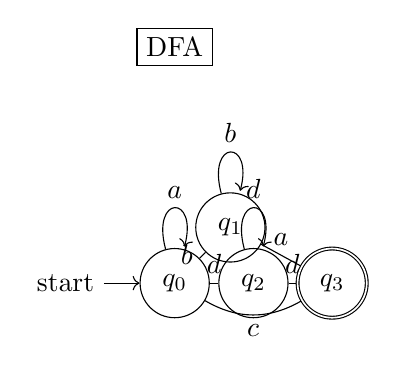
\begin{tikzpicture}
						\node[draw] at (0,3) {DFA};
						\node[state, initial] (q0) {$q_0$};
						\node[state, above right of=q0] (q1) {$q_1$};
						\node[state, right of=q0] (q2) {$q_2$};
						\node[state, accepting, right of=q2] (q3) {$q_3$};
						\draw (q0) edge[loop above] node{$a$} (q0)
						(q0) edge[bend right,below] node{$c$} (q3)
						(q0) edge[left] node{$b$} (q1)
						(q1) edge[loop above] node{$b$} (q1)
						(q2) edge[loop above] node{$d$} (q1)
						(q1) edge[above] node{$a$} (q3)
						(q0) edge[right, above] node{$d$} (q2)
						(q2) edge[right, above] node{$d$} (q3)
						;
					\end{tikzpicture}
				}
				\caption{FSM diagram of \texttt{a*(b+a|d*c) regular expression}}
				\label{fig:regex_FSA}
			\end{figure}
		\end{column}
	\end{columns}
\end{frame}



\section{Analysis}
\subsection{Related work}
\begin{frame}[fragile=singleslide]\frametitle{Related work}
	\begin{table}[htbp]
		\centering
		\scalebox{0.75}{
			\begin{tabular}{|l|c|}
				\hline
				\textbf{Study}                                                            & \textbf{Year} \\
				\hline
				\multicolumn{2}{|c|}{\textbf{FSA measurements}}                                           \\
				\hline
				GPU Acceleration of Regular Expression \cite{Becchi:regex_large_dataset}  & 2013          \\
				\hline
				\multicolumn{2}{|c|}{\textbf{Acceleration platforms}}                                     \\
				\hline
				Demystifying Automata Processing \cite{Nourian:DemystifyingFSA}           & 2017          \\
				\hline
				\multicolumn{2}{|c|}{\textbf{Papers on speeding up FSA processing on GPUs}}               \\
				\hline
				\multicolumn{2}{|c|}{\textbf{DFA}}                                                        \\
				\hline
				On-the-Fly Principled Speculation \cite{zhao2015fly}                      & 2015          \\
				\hline
				Scaling Out Speculative Execution \cite{Xia:FSA-scaling}                  & 2020          \\
				\hline
				GSpecPal: Speculation-Centric FSM Parallelization \cite{wang2022gspecpal} & 2022          \\
				\hline
				\multicolumn{2}{|c|}{\textbf{NFA}}                                                        \\
				\hline
				Why GPUs are Slow at Executing NFAs \cite{Liu:WhyGPUSlowNFA}              & 2020          \\
				\hline
				Asynchronous Automata Processing on GPUs \cite{Liu:Asynchronous}          & 2023          \\
				\hline
			\end{tabular}
		}
		\caption{Table of Papers on Regular Expression Matching}
		\label{tab:papers}
	\end{table}
\end{frame}

\subsection{Studies findings}
\begin{frame}[fragile=singleslide]\frametitle{Studies findings: FSA}

\end{frame}

\begin{frame}[fragile=singleslide]\frametitle{Studies findings: Acceleration platforms}

\end{frame}













\section*{Conclusion and future work}
% hviezdička zabezpečí, aby sa táto časť neocitla v prehľade prezentácie - každá prezentácia má zhodnotenie a prehľad by sa tým zbytočne zahlcoval

\begin{frame}[fragile=singleslide]\frametitle{Conclusion and future work}
	\begin{itemize}
		\item Každá prezentácia musí byť nejako uzavretá
		\item Ale vždy je čo robiť ďalej\ldots{}
	\end{itemize}
\end{frame}

\begin{frame}[fragile=singleslide]\frametitle{Bibliography}
	\fontsize{4.5}{1}
	\bibliography{zdroje}
	\bibliographystyle{plain}
\end{frame}



\end{document}

\section*{TEST}
% hviezdička zabezpečí, aby sa táto časť neocitla v prehľade prezentácie - každá prezentácia má zhodnotenie a prehľad by sa tým zbytočne zahlcoval

\begin{frame}[fragile=singleslide]\frametitle{Test}
	\begin{table}
		\begin{tabular}{l | c | c | c | c }
			Competitor Name & Swim  & Cycle & Run   & Total \\
			\hline \hline
			John T          & 13:04 & 24:15 & 18:34 & 55:53 \\
			Norman P        & 8:00  & 22:45 & 23:02 & 53:47 \\
			Alex K          & 14:00 & 28:00 & n/a   & n/a   \\
			Sarah H         & 9:22  & 21:10 & 24:03 & 54:35
		\end{tabular}
		\caption{Triathlon results}
	\end{table}
\end{frame}

\begin{frame}[fragile=singleslide]\frametitle{Test2}
	\frametitle{Pictures}
	\begin{figure}
		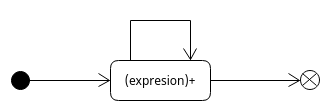
\includegraphics[scale=0.5]{Diagram2.png}
		\caption{test}
	\end{figure}
	adfklajdfadvafgsfbsg
\end{frame}






Text \end{document} za príkazom \end{document} LaTeX ignoruje, takže tu môžete odkladať veci (aj celé slajdy), ktoré nechcete vymazať, lebo ich ešte možno budete potrebovať, avšak ich v danom momente nechcete mať v slajdoch.
